\documentclass[12pt]{article}

\usepackage{amsmath}
\usepackage{amssymb}
\usepackage{amsthm}
\usepackage{centernot}
\usepackage{fullpage}
\usepackage{makecell}
\usepackage{tabularx}
\usepackage[hypcap=false]{caption}
\usepackage{tikz, tkz-euclide}
\usetikzlibrary{decorations.pathreplacing,arrows}
\usetikzlibrary{quotes,angles,calc,intersections}

\usepackage{titling}
\usepackage{pdfpages}
\usepackage{enumitem}
\usepackage{multicol}
\usepackage{bm}

\usepackage{linear}
\usepackage{common}

\begin{document}

\title{Abstract Algebra}
\author{Brendan Burkhart}
\maketitle

\tableofcontents
\newpage

\section{Symmetries}

Our first motivation for studying groups will be the symmetries of regular $n$-gons, starting with the regular $3$-gon: the equilateral triangle. The symmetries of a regular $n$-gon in the plane are rotations and reflections which take the $n$-gon to itself.

For example, if we take an equilateral triangle and label the vertices $A, B, C$, in anti-clockwise order starting from the top, we have two rotational symmetries: rotation by $120^\circ$ and rotation by $240^\circ$, in a particular sense or direction, say anti-clockwise. We also have three reflection symmetries -- reflections across a line going from one vertex to the midpoint of the opposite edge.

\begin{figure}[ht!]
    \centering
    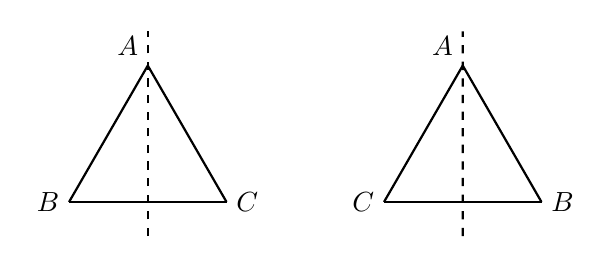
\begin{tikzpicture}
        \coordinate (A1) at (0, {sqrt(3)});
        \coordinate (B1) at (-1, 0);
        \coordinate (C1) at (1, 0);
        \coordinate (R1) at ($(B1)!0.5!(C1)$);
        \coordinate (R11) at ($(A1)!1.25!(R1)$);
        \coordinate (R12) at ($(R1)!1.25!(A1)$);

        \node[anchor=south east] at (A1) {$A$};
        \node[anchor=east] at (B1) {$B$};
        \node[anchor=west] at (C1) {$C$};

        \draw [thick] (A1)--(B1);
        \draw [thick] (B1)--(C1);
        \draw [thick] (C1)--(A1);

        \draw [thick, dashed] (R11)--(R12);

        \coordinate (A2) at (4, {sqrt(3)});
        \coordinate (B2) at (5, 0);
        \coordinate (C2) at (3, 0);
        \coordinate (R2) at ($(B2)!0.5!(C2)$);
        \coordinate (R21) at ($(A2)!1.25!(R2)$);
        \coordinate (R22) at ($(R2)!1.25!(A2)$);

        \node[anchor=south east] at (A2) {$A$};
        \node[anchor=west] at (B2) {$B$};
        \node[anchor=east] at (C2) {$C$};

        \draw [thick] (A2)--(B2);
        \draw [thick] (B2)--(C2);
        \draw [thick] (C2)--(A2);

        \draw [thick, dashed] (R21)--(R22);
    \end{tikzpicture}
\caption{Reflection symmetry $S_1$}
\label{fig:triangle-reflection}
\end{figure}

Let $R$ be the rotation by $120^\circ$ anti-clockwise. Then the rotation by $240^\circ$ anti-clockwise is simply $R$ applied twice, so we will denote it by $R^2$. Let $S_1$ be the reflection symmetry across the line through the top vertex, $S_2$ across the line through the left vertex, and $S_2$ the right vertex. The final symmetry is the identity transform, which we will call $e$. The triangle therefore has six symmetries in total: $\{e, S_1, S_2, R, R^2\}$.

\begin{figure}[ht!]
    \centering
    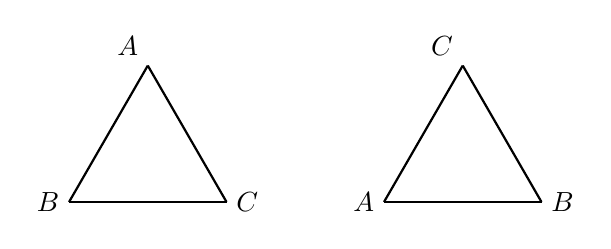
\begin{tikzpicture}
        \coordinate (A1) at (0, {sqrt(3)});
        \coordinate (B1) at (-1, 0);
        \coordinate (C1) at (1, 0);

        \node[anchor=south east] at (A1) {$A$};
        \node[anchor=east] at (B1) {$B$};
        \node[anchor=west] at (C1) {$C$};

        \draw [thick] (A1)--(B1);
        \draw [thick] (B1)--(C1);
        \draw [thick] (C1)--(A1);

        \coordinate (A2) at (3, 0);
        \coordinate (B2) at (5, 0);
        \coordinate (C2) at (4, {sqrt(3)});

        \node[anchor=east] at (A2) {$A$};
        \node[anchor=west] at (B2) {$B$};
        \node[anchor=south east] at (C2) {$C$};

        \draw [thick] (A2)--(B2);
        \draw [thick] (B2)--(C2);
        \draw [thick] (C2)--(A2);
    \end{tikzpicture}
\caption{Rotation symmetry $R$}
\label{fig:triangle-rotation}
\end{figure}

Since every symmetry takes the triangle to itself, products (compositions) of Symmetries are themselves symmetries. If $u$ and $w$ are symmetries, let $uw$ denote the composition of first $w$ and then $u$ after the manner of function composition. For example, $S_1S_2 = R$, $RR = R^2$, and $R^2R = e$.

Note that multiplication of symmetries is not necessarily commutative: $S_1S_2 = R$, but $S_2S_1 = R^2$. Multiplication with the identity is however commutative: $eR^2 = R^2 = R^2e$, etc.

We can construct a full multiplication table for the six symmetries of the $3$-gon listing all possible binary products, which is shown in Table \ref{triangle-multiplication-table}.

\begin{minipage}{\linewidth}
    \begin{center}
    \captionof{table}{Group multiplication table for $3$-gon}
    \label{triangle-multiplication-table}
    \begin{tabular}{|c||c|c|c|c|c|c|}
    \hline
    \thead{$\circ$} & \thead{$e$} & \thead{$S_1$} & \thead{$S_2$} & \thead{$S_3$} & \thead{$R$} & \thead{$R^2$}\\
    \hline\hline
    $e$   & $e$   & $S_1$ & $S_2$ & $S_3$ & $R$   & $R^2$ \\ \hline
    $S_1$ & $S_1$ & $e$   & $R$   & $R^2$ & $S_2$ & $S_3$ \\ \hline
    $S_2$ & $S_2$ & $R^2$ & $e$   & $R$   & $S_3$ & $S_1$ \\ \hline
    $S_3$ & $S_3$ & $R$   & $R^2$ & $e$   & $S_1$ & $S_2$ \\ \hline
    $R$   & $R$   & $S_3$ & $e$   & $S_2$ & $R^2$ & $e$   \\ \hline
    $R^2$ & $R^2$ & $S_2$ & $S_3$ & $S_1$ & $e$   & $R$   \\ \hline
    \end{tabular}
    \end{center}
\end{minipage}

\end{document}
